\section{Χρονική ολοκλήρωση των αεροελαστικών εξισώσεων}

Η χρονική απόκριση των δυο βαθμών ελευθερίας εκφράζονται ως εξής:

\begin{equation}
    \mathbf{x}(t) = \mathbf{x}_{hom} + \mathbf{x}_{part}
    \label{eq:timesol}
\end{equation}

Όπου $\mathbf{x}_{hom}$ η ομογενής λύση του συστήματος και $\mathbf{x}_{part}$ η μερική λύση που ακολουθεί τη μορφή της διέγερσης -- των αεροδυναμικών φορτίων.

Η ομογενής λύση, χρησιμοποιώντας τον ιδιοανυσματικό μετασχηματισμό είναι:

\begin{equation}
    \mathbf{x}(t)_{hom} = \sum_{k=1}^2\Bigg[\phi_{0k}e^{Re(\lambda_k)}\Big(A_kcos(Im(\lambda_k)t+\theta_k)+B_ksin(Im(\lambda_k)t+\theta_k)\Big)\Bigg]
    \label{eq:homogenous}
\end{equation}

Όπου, με k συμβολίζουμε την k-oστή ιδιοτιμή, $\phi_{0k}$ είναι το μέτρο της μιγαδικής ιδιομορφής και $\theta_k$ η φάση της. Δηλαδή, η ομογενής λύση προκύπτει απο υπέρθεση των ταλαντώσεων για όλες τις ιδιοτιμές. Οι συντελεστές $A_k, B_k$ προσδιορίζονται απο τις αρχικές συνθήκες. 

Η αντίστοιχη μερική λύση, θεωρώντας σταθερά αεροδυναμικά φορτία είναι η μόνιμη απόκριση του συστήματος και είναι:

\begin{equation}
    \mathbf{x}_{part} = \begin{bmatrix}
    \mathbf{0} & \mathbf{0}\\
    \mathbf{0} & \mathbf{K}^{-1}
    \end{bmatrix}
    \cdot
    \begin{Bmatrix}
    0\\0\\F_x\\F_z
    \end{Bmatrix}
    \label{eq:partial}
\end{equation}

Επομένως, με δεδομένα τα παραπάνω, μπορούμε να προσδιορίσουμε την απόκριση του συστήματος. Για την περίπτωση της μόνιμης ροής, γραμμικοποιήσαμε γύρω απο τη θέση ισορροπίας, και χρησιμοποιήσαμε τις παραπάνω εξισώσεις για τον υπολογισμό της χρονοσειράς της απόκρισης, με απόσβεση και σταθερό αεροδυναμικό φορτίο όπως υπολογίζεται στη θέση αναφοράς.

Για την περίπτωση της μη-μονιμης ροής, όπως αναφέραμε και σε προηγούμενη παράγραφο, επειδή για τον υπολογισμό των αεροδυναμικών φορτίων απαιτείται η επίλυση μιας ακόμη διαφορικής εξίσωσης, σε κάθε χρονικό βήμα, με αρχική συνθήκη την κατάσταση του προηγούμενου βήματος, υπολογίζουμε τα αεροδυναμικά φορτία, και προσδιορίζουμε τη νεα κατάσταση απο τις \crefrange{eq:timesol}{eq:partial}. Εδώ κάνουμε την απλούστευση πως για τη διάρκεια κάθε βήματος, τα αεροδυναμικά φορτία είναι σταθερά και υπολογίζουμε τη μερική λύση απο την \cref{eq:partial}. Επιπλέον, σε αυτή την περίπτωση, στην ομογενή λύση χρησιμοποιούμε μηδενικό μητρώο απόσβεσης, αφού η απόσβεση υπεισέρχεται έμμεσα απο την μεταβολή των αεροδυναμικών φορτίων ανάλογα της κατάστασης του συστήματος. 

Ξεκινώντας με μηδενικές μετατοπίσεις, ταχύτητες, και επιταχύνσεις, και χρησιμοποιώντας τα δεδομένα όπως παρατίθενται στον πίνακα \ref{tab:data}, η χρονοσειρά της απόκρισης για μόνιμη και μη-μόνιμη ροή, φαίνονται στα \crefrange{fig:responseu}{fig:responsew}.

\begin{figure}[ht!]
    \begin{center}
        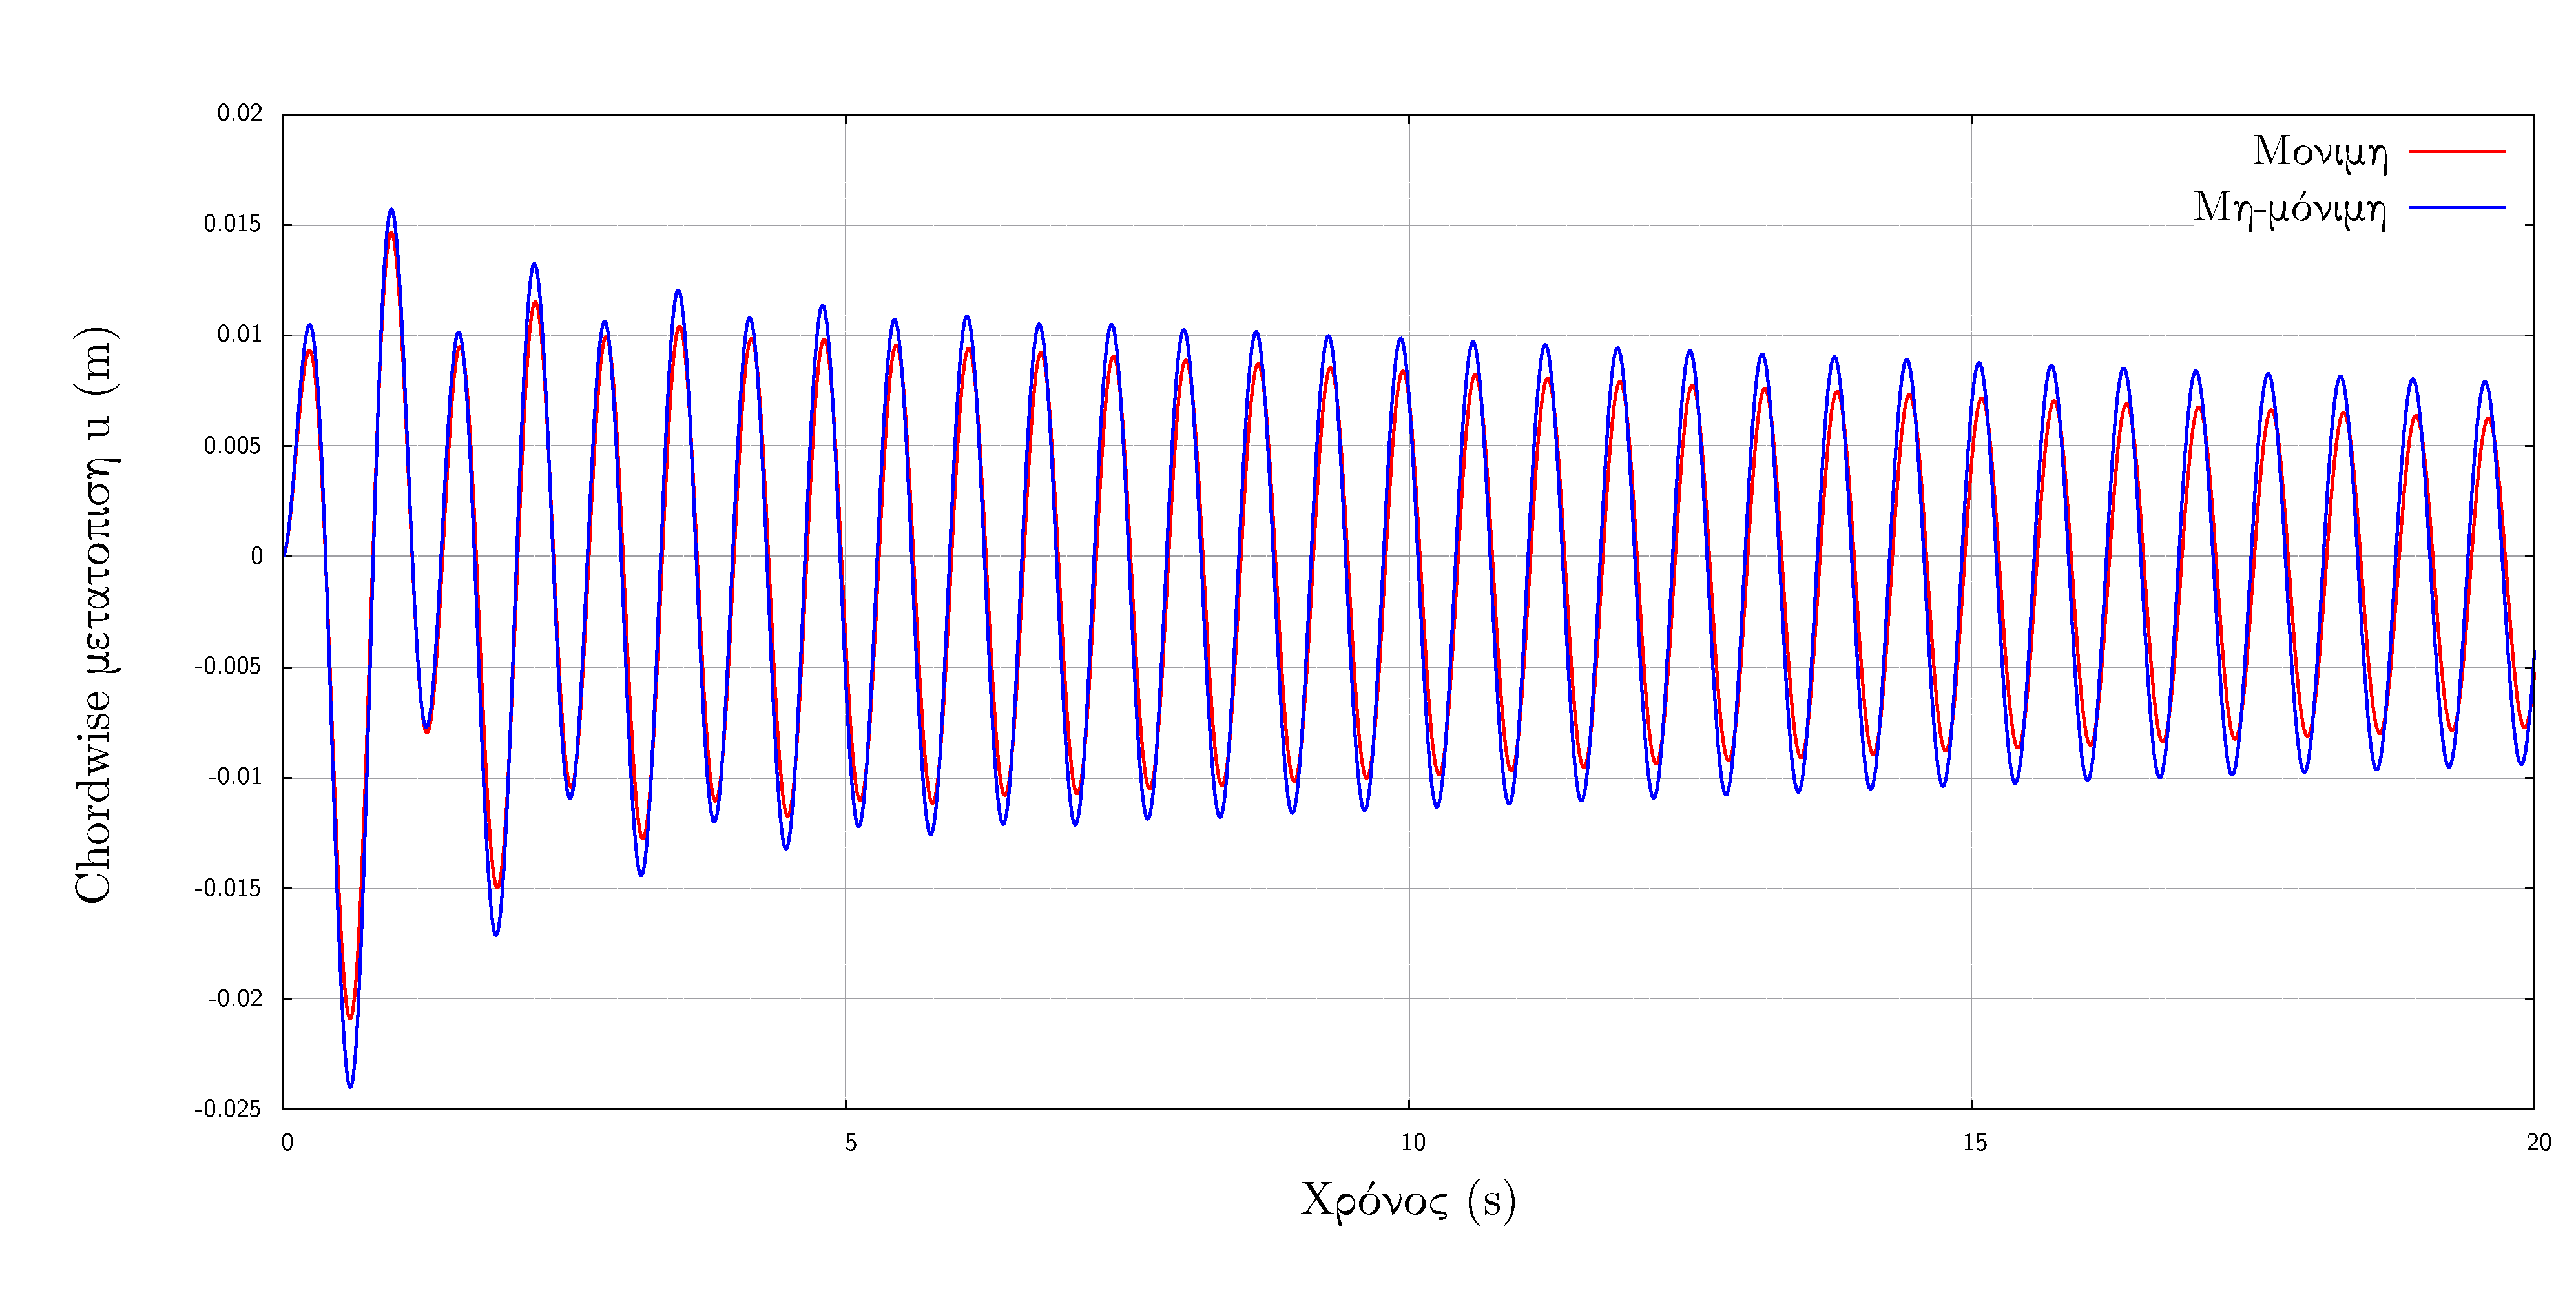
\includegraphics[width=0.95\textwidth]{./figures/time_u.pdf}
    \end{center}
    \caption{Χρονοσειρά απόκρισης -- μετατόπιση u}
    \label{fig:responseu}
\end{figure}

\begin{figure}[ht!]
    \begin{center}
        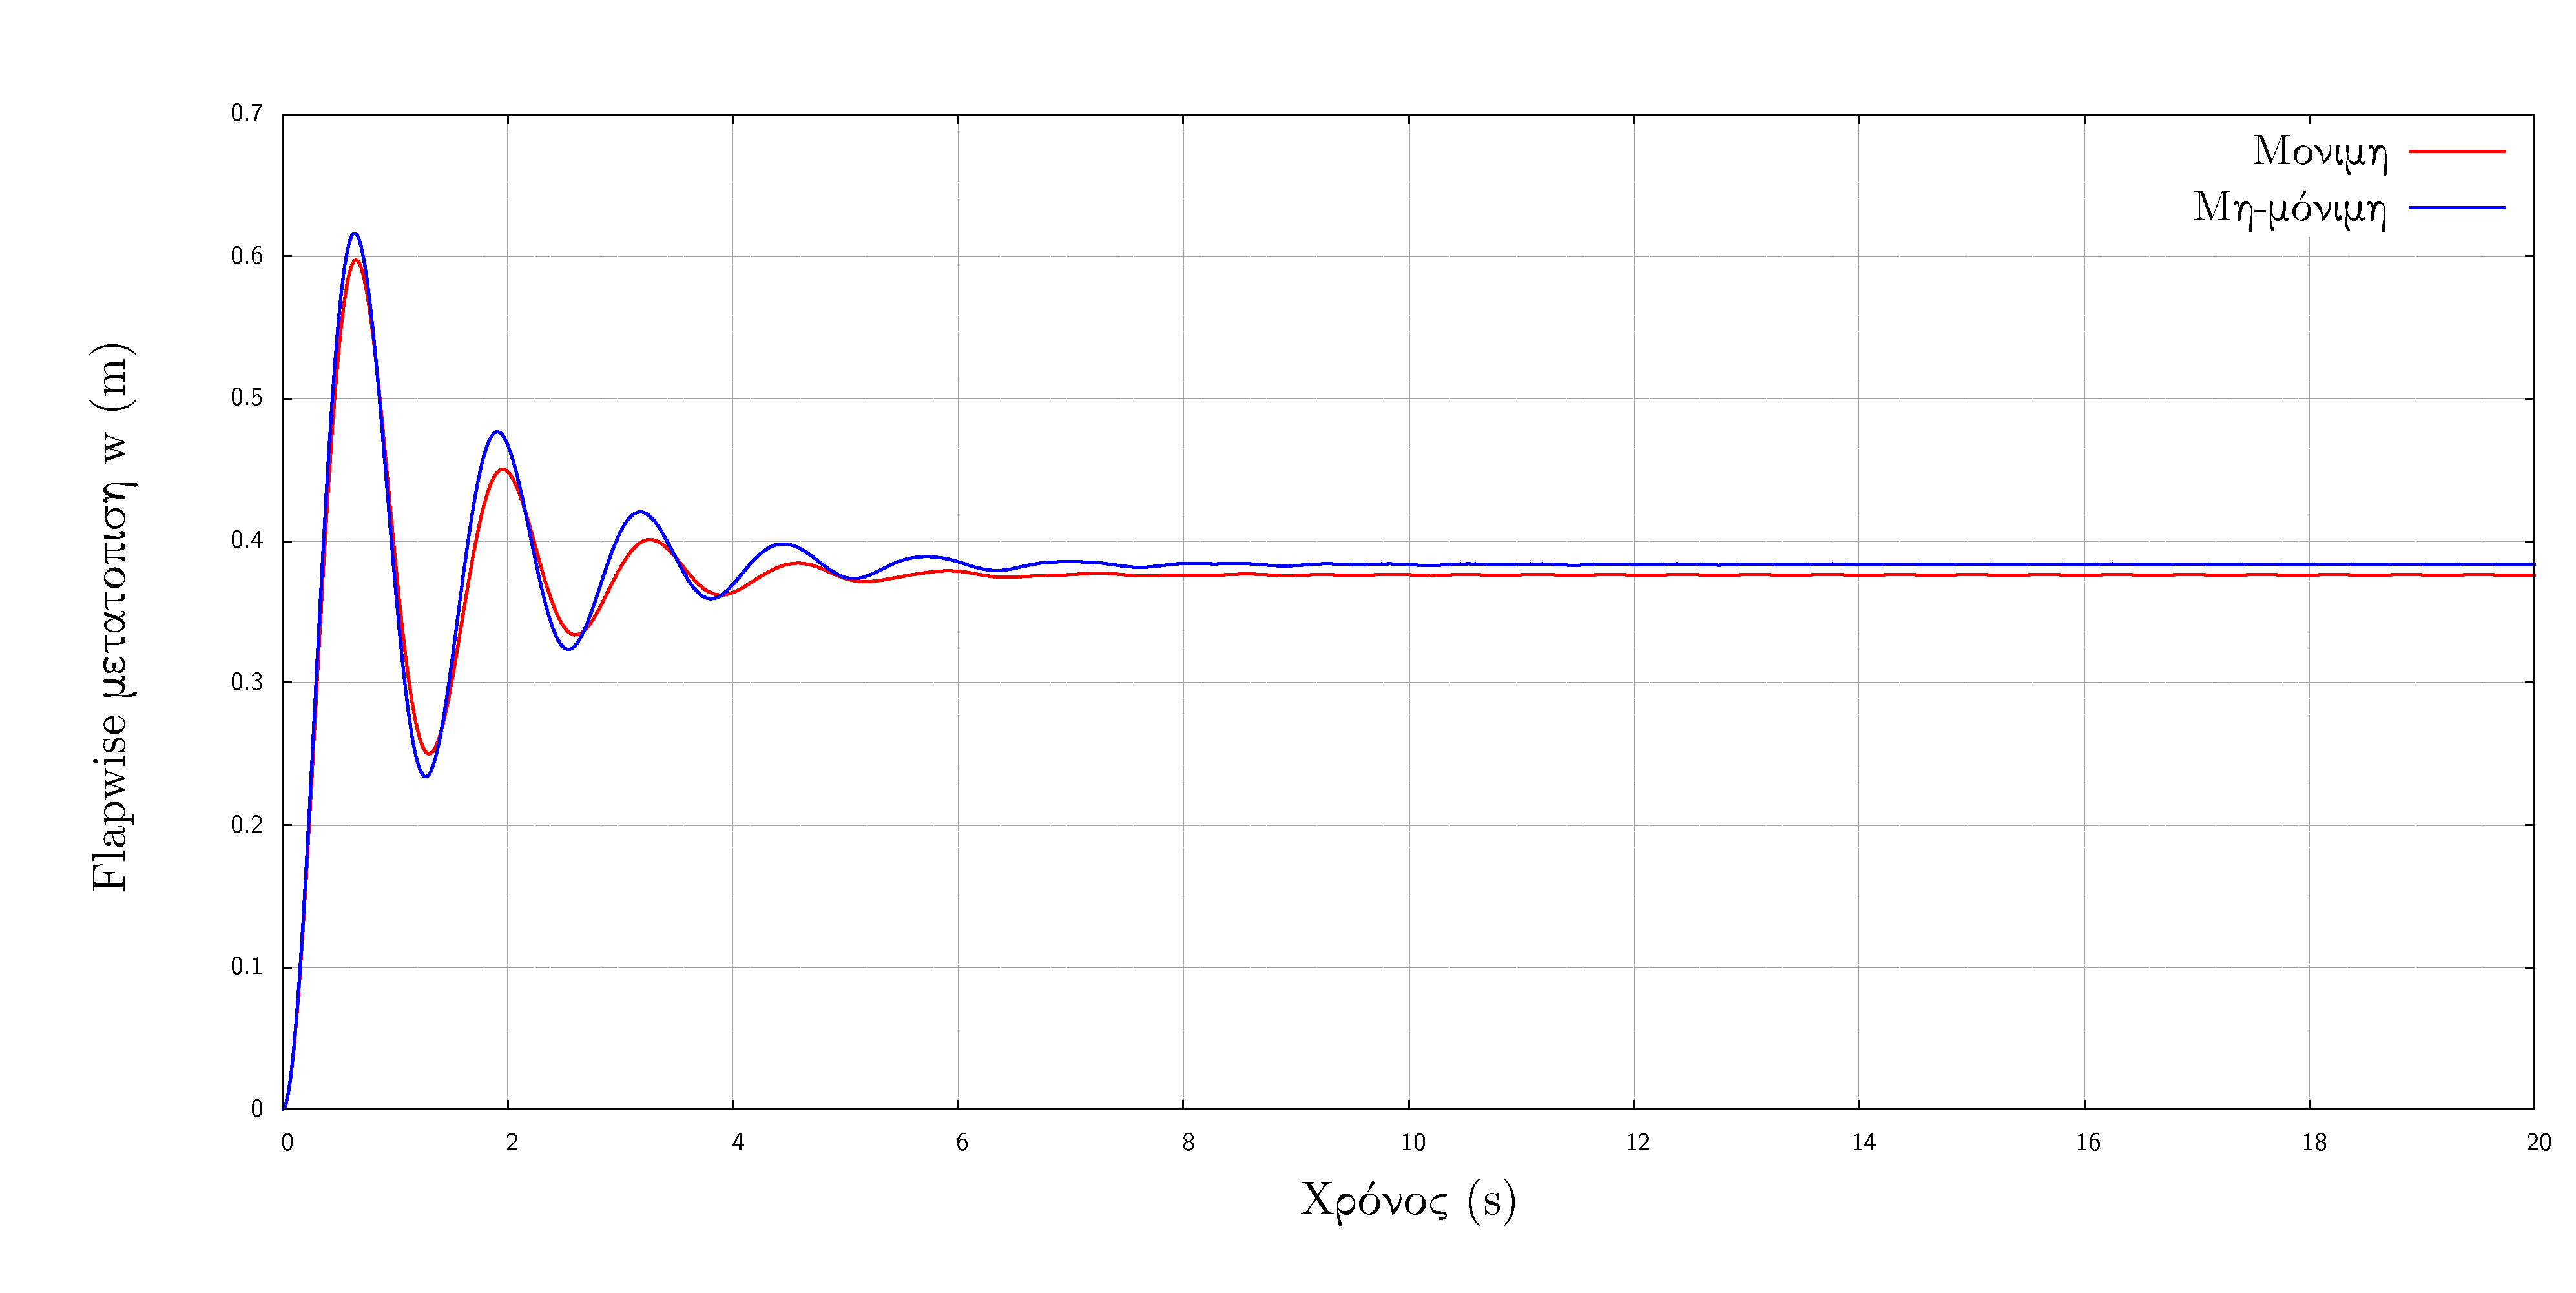
\includegraphics[width=0.95\textwidth]{./figures/time_w.pdf}
    \end{center}
    \caption{Χρονοσειρά απόκρισης -- μετατόπιση w}
    \label{fig:responsew}
\end{figure}

\newpage
Παρατηρούμε πως τα δυο μοντέλα παρέχουν κοντινές αποκρίσεις. Επιπλέον, ειναι προφανές πως κατά την chordwise διεύθυνση έχουμε πολύ μικρότερη απόσβεση, σημειώνοντας πως για χρόνο t=20s η ταλάντωση έχει αποσβεσθεί ελάχιστα. Αντίθετα, όπως υποδεικνύουν και οι τιμές της απόσβεσης που προκύπτουν απο την ιδιανυσματική ανάλυση, κατά την διεύθυνση πτερύγησης έχουμε πολύ εντονότερη απόσβεση. Το γεγονός οτι έχουμε πολύ ασθενή σύζευξη μεταξύ των δυο βαθμών ελευθερίας συντελεί στην ασθενή απόσβεση στη μετατόπιση u. Αν είχαμε εντονότερη σύζευξη, είτε επιλέγοντας μεγαλύτερη γωνία $\theta$ ή καλύτερα τροποποιώντας τη διατομή της πτέρυγας ώστε να τροποποιήσουμε τους κύριους άξονες, τότε η ταλάντωση στην chordwise διεύθυνση θα αποσβαινόταν πολύ γρηγορότερα, επάγοντας μετατοπίσεις στην flapwise διεύθυνση όπου έχουμε υψηλή απόσβεση.

Αναφορικά με τη σύγκριση των αποτελεσμάτων των δυο μοντέλων, αρχικά αναφέρεται πως η προσέγγιση της συμπεριφοράς $C_L$ ως γραμμική δίνει ελαφρά διαφορετικές τιμές συγκριτικά με την καμπύλη της μόνιμης ροής, και κατοπτρίζεται σε ελαφρά διαφορετικό σημείο ισορροπίας όταν αποσβαίνεται η ταλάντωση, ωστόσο θα μπορούσε να αντιμετωπισθεί με πιο ακριβή προσδιορισμό της κλίσης της γραμμικής περιοχής του $C_L$ και του σημείου $\alpha_0$. Επιπλέον, το μοντέλο μη-μόνιμης ροής φαίνεται να είναι πιο συντηρητικό συγκριτικά με τη μόνιμη ροή, αφού παρατηρούμε μεγαλύτερα πλάτη ταλάντωσης, ωστόσο στη συγκεκριμένη περίπτωση μπορεί να οφείλεται στην ελαφρώς μεγαλύτερη τιμή του $C_L$ όπως αναφέραμε παραπάνω. 


\label{TextLastPage}
%\afterpage
